\section{\hspace{1em}Въведение}
\begin{frame}[t]{Термини от епидемологията}
  \begin{itemize}
    \item Патоген е причинител на зараза (напр. вирус, бактерия, прион).
    \item Вектор е носител на патоген, който може да зарази други индивиди.
    \item S (Susceptible - Податливи) - податливи са тези, които не носят патогена и могат да бъдат заразени с него
    \item I (Infected - Заразени) - заразени са носители на патогена
    \item Заболяване има ендемичен характер, когато има (приблизително) константен ненулев брой заразени.
  \end{itemize}
\end{frame}

\begin{frame}[t]{Малария}
  Симптоми са периодичен пароксизъм(продължителни спазми, потене, треска), умора, главоболие, хепатомегалия (разрастнал се черен дроб), белодробен оток, анемия (намалено количество еритроцити), мозъчек оток, смърт.

  Патогенът е един 4 вида от рода \textit{Plasmodium} маларийни плазмодии, които са едноклетъчни еукариоти, т.е. едноклетъчни с ядро. Интензивността на симптомите зависи от вида плазмодий.

  В края на XIX век Ross доказва, че вектора на маларията са комарите от род \textit{Anopheles}.
  В началото на XX век моделира маларията с две диференциални уравнения, като модела му е основа за моделирането на векторнопредавани заболявания и до днес.
\end{frame}

\begin{frame}[t]{Разпространение на маларията}
  Хората могат да оздравеят, като оранизмът им се прочисти от плазмодиите.
  Не развиват траен имунитет, но обикновено повторни заболявания се претърпяват по-лесно.

  Комарите са насекоми и нямат имунна система, така че не могат да се предпазват от паразити.

  Затова в моделите на Ross динамиката се описва чрез прехода между класове:
  \begin{itemize}
    \item $S \rightarrow I \rightarrow S$ (SIS) при хората
    \item $S \rightarrow I$ (SI) при комарите
  \end{itemize}

  \begin{figure}
    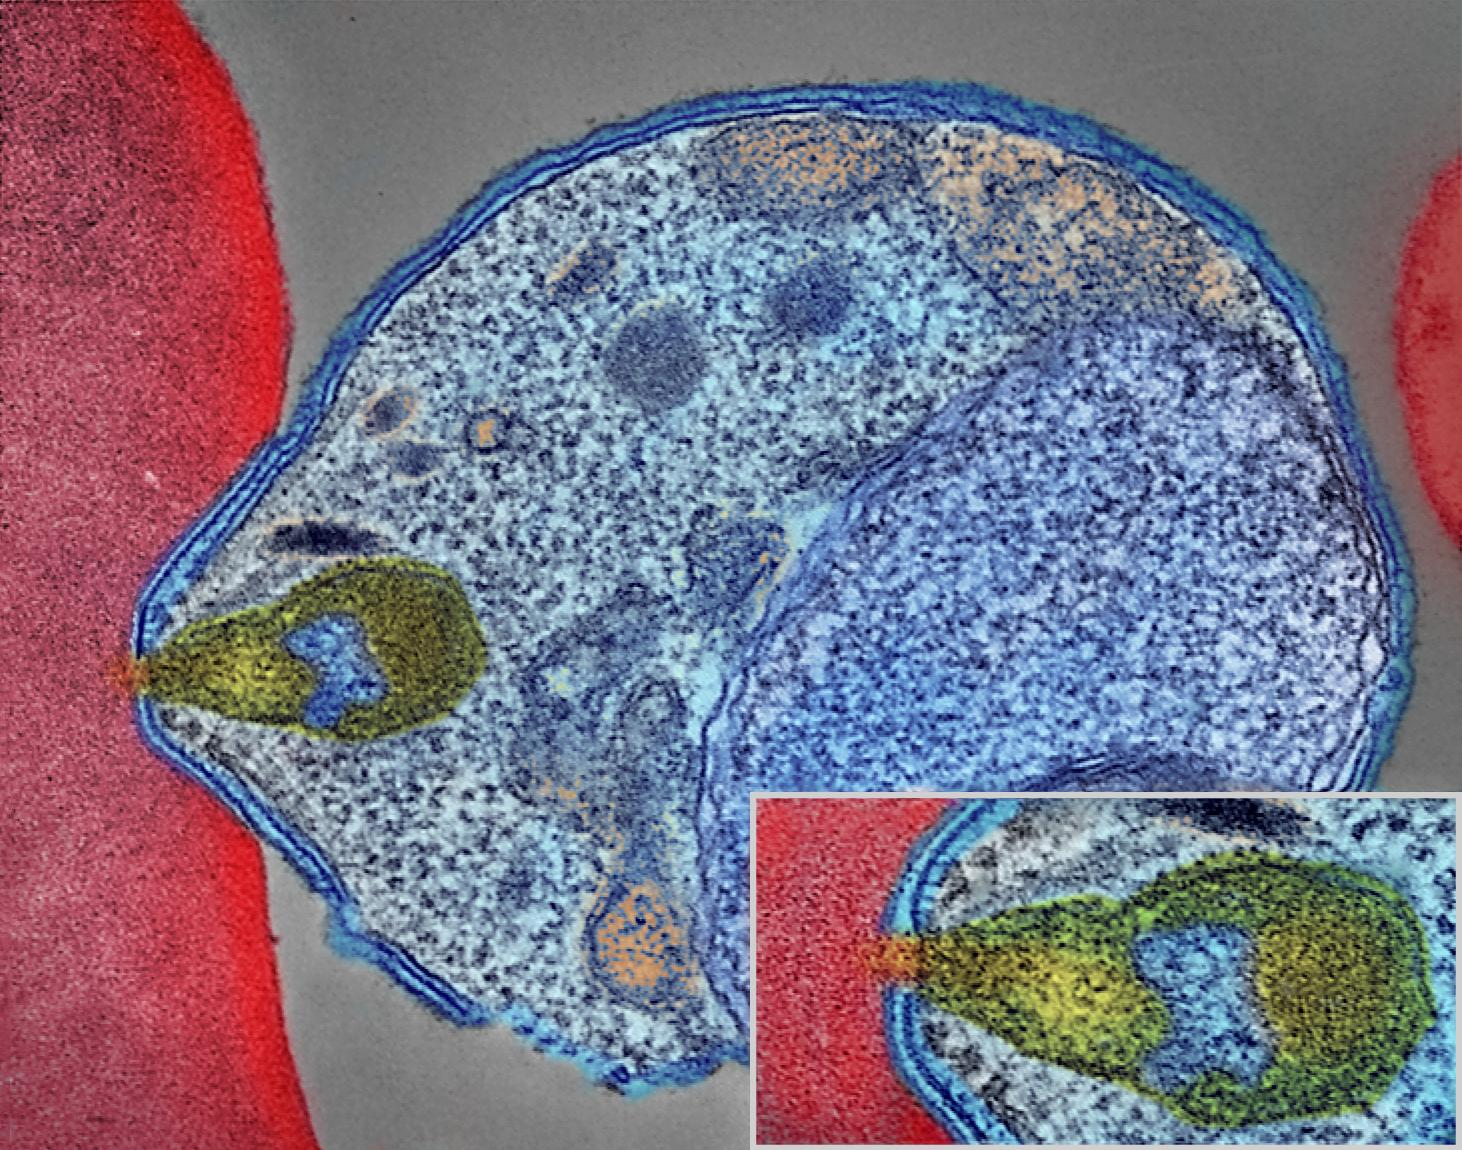
\includegraphics[height=0.3\textheight]{Malaria_Parasite_Connecting_to_Human_Red_Blood_Cell_(34034143483).jpg}
    \centering
    \caption{Оцветена снимка от електронен микроскопскоп на плазмодий нападащ еритроцит}
  \end{figure}
\end{frame}
